\documentclass[twocolumn]{article}
\usepackage{graphicx}
\usepackage{amsmath}
\usepackage{amssymb}
\usepackage[top=1.5cm, bottom=1.5cm, left=1.6cm, right=1.6cm]{geometry}
\usepackage{float}
\usepackage{stfloats}  % 放在 preamble 區域
\usepackage{multirow}
\usepackage{makecell}

\title{PLNTP: Pulse Localization Network with Temporal Prior}
\begin{document}
\author{%
  Guanhao Huang$^{1}$, Hong Lu$^{1}$\\[0.5ex]
  {\small $^{1}$Shanghai Key Laboratory of Intel. Info. Processing,
    School of Computer Science,}\\
  {\small Fudan University, P.R.China}%
}
\date{}
\maketitle

\begin{abstract}
Accurately locating the positions of cun, guan, and chi is a crucial step in pulse diagnosis during palpation. To address this, various methods have been proposed to improve the precision of pulse point localization. In recent years, deep-learning-based approaches have shown remarkable success in keypoint detection tasks, offering advantages such as high localization accuracy, simplified experimental setups, and ease of integration into mechanical systems. In this paper, we explore the use of a temporal attention mechanism to extract spatiotemporal features from infrared video data, aiming to enhance localization accuracy. We propose a heatmap-based method that incorporates a temporal attention prior, which captures subtle temporal variations to guide the model in learning more discriminative features of the pulse locations. Experimental results demonstrate that our method achieves localization accuracies of 97.966\%, 97.288\%, and 97.627\% for cun, guan, and chi, respectively, under a 100-pixel (10 mm) threshold. Even at a fine-grained threshold of 20 pixels (2 mm), the accuracies remain at 24.407\%, 26.441\%, and 21.356\%, respectively. These results highlight the promising potential of combining computer vision and Traditional Chinese Medicine for the development of intelligent medical systems.
\end{abstract}
% 2025--07-21

\section{Introduction}
Traditional Chinese Medicine (TCM) has a long-standing history in China and is a medical system developed through centuries of empirical practice and clinical observation. Among various diagnostic techniques, palpation is a fundamental method used by TCM practitioners to assess a patient’s condition. During palpation, the practitioner presses their fingers on three pulse positions on the wrist—namely, cun, guan, and chi—to analyze potential abnormalities.

However, the localization of these pulse positions heavily depends on individual experience, leading to subjectivity and inconsistency among practitioners. Moreover, external finger pressure can alter the pulse signal, introducing deviations from the actual pulse characteristics. As a result, the objectification of palpation has become an emerging area of research within TCM. To address this, researchers have developed pulse diagnosis instruments to simulate the palpation process in a more standardized and quantifiable manner.

Accurate localization of pulse positions is a critical step in such systems, and various methods have been proposed to achieve this goal. These methods can be broadly categorized into sensor-based, image-processing-based, and deep-learning-based approaches.

Sensor-based methods employ various types of sensors—such as pressure sensors, piezoelectric sensors, and photometric sensors—to capture physiological signals. For example, Chen et al.~\cite{chen2015} employed optical triangulation, projecting infrared light onto the wrist and capturing its variations using CMOS sensors; the location with the strongest variation was identified as the pulse point. Yang et al.~\cite{yang2017} used a CSRR sensor array to detect changes in the electric field. Wang et al.~\cite{wang2014} first applied principles from Chinese Medicine theory to estimate the approximate positions of the pulse points, then used dedicated probes for each of the cun, guan, and chi points for further refinement.

Image-processing-based methods rely on traditional computer vision techniques, such as edge detection, often combined with TCM theory~\cite{geng2020}, to estimate pulse locations.

Deep-learning-based methods utilize neural networks to learn discriminative wrist features and infer the pulse positions. Among the three categories, deep learning has demonstrated the most promising results in terms of localization accuracy. These models learn diverse spatial and contextual representations from large datasets annotated with keypoint labels, enabling more robust and precise pulse localization.
% 2025-07-28

\section{Related Work}
Luo et al.~\cite{luo2019} proposed a two-stream convolutional neural network (CNN), where one stream processes RGB images and the other processes imaging photoplethysmography (iPPG) images. Features from both streams are extracted independently and fused at a middle layer before regressing the coordinates of the cun point. This work was the first to explore the potential of deep-learning-based pulse localization with promising accuracy. However, its performance is limited by the influence of environmental lighting, making it difficult to achieve further improvements.

\begin{figure*}[!t]
  \centering
  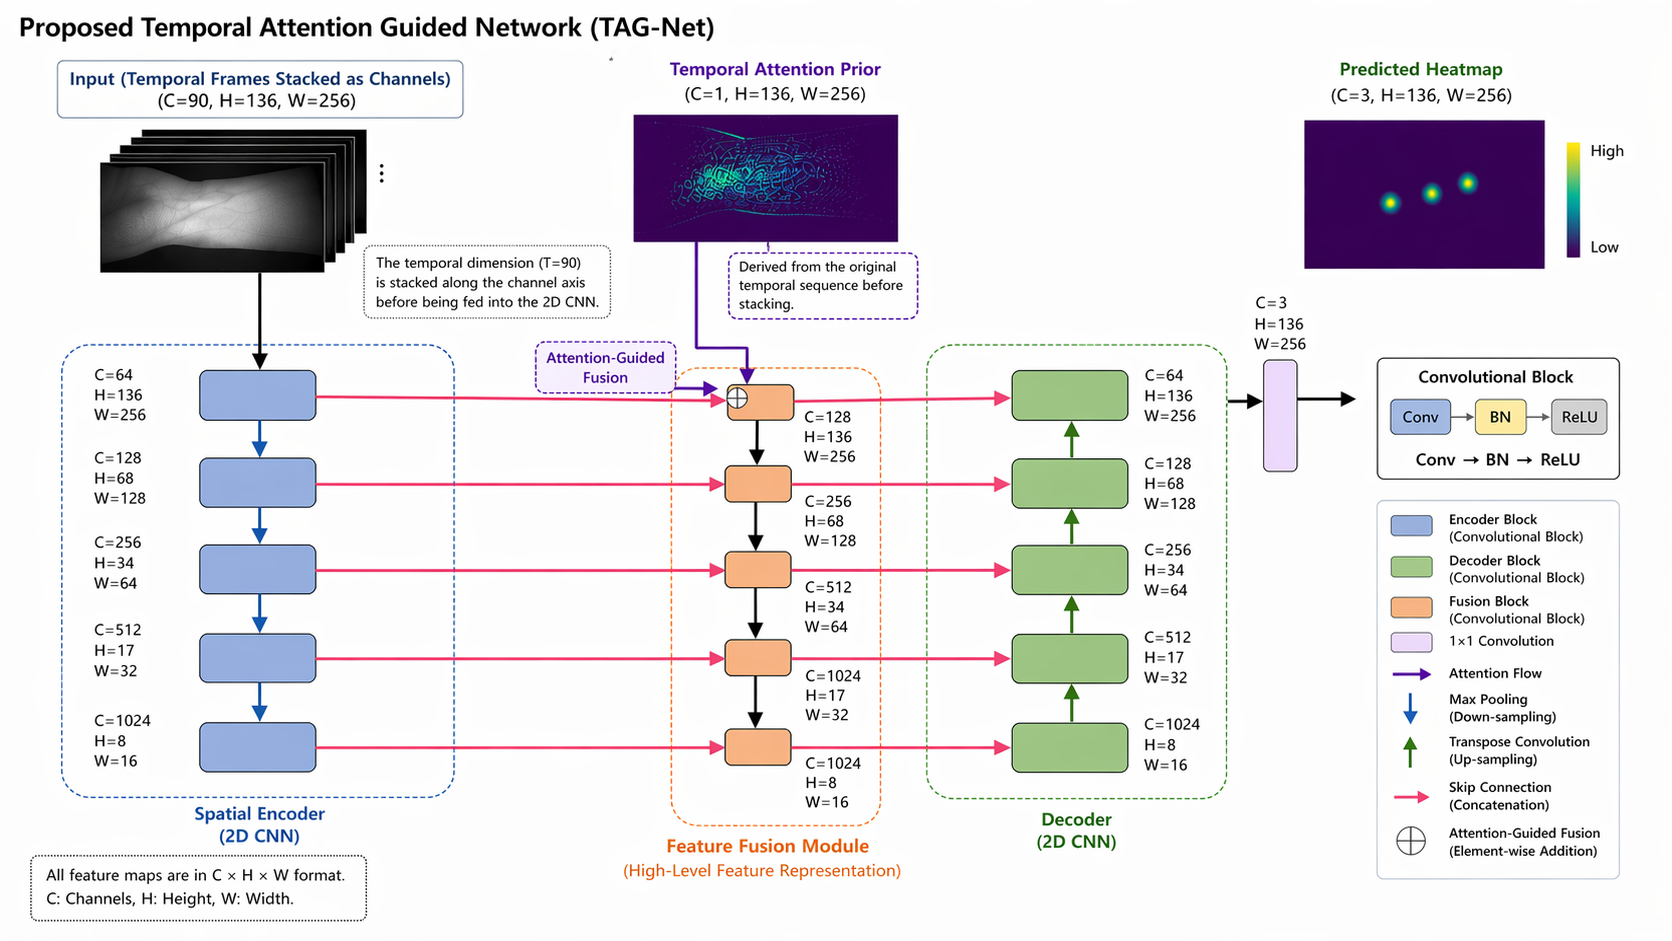
\includegraphics[width=\textwidth, keepaspectratio]{figures/network-structure.png}
  \caption{Network architecture of PLNTP.}
  \label{PLNTP}
\end{figure*}

Yang et al.~\cite{yang2021} introduced the Pulse Localization Network (PLN), a seven-layer CNN that uses infrared images as input to mitigate the impact of ambient light. While this approach allows the network to converge more easily, the use of still images fails to capture the subtle temporal characteristics of pulse signals.

Yang et al.~\cite{yang2022} proposed the Spoon Fully Convolutional Network (SFCN), a heatmap-based architecture inspired by U-Net~\cite{ronneberger2015}. SFCN performs three upsampling operations, resulting in an output heatmap at half the input resolution. They also incorporated attention modules into the skip connections to enhance localization accuracy. This method offered a new direction for pulse localization, achieving higher accuracy under small thresholds. However, due to the relatively low image resolution, it struggles to deliver precise localization on high-resolution inputs.

Chen et al.~\cite{chen2022} presented a 3D CNN-based framework using infrared video instead of static images. The temporal information in the video captures subtle, otherwise invisible, vibrations of the pulse position, providing additional cues for localization. While their approach introduced the innovative idea of utilizing temporal features, the simplicity of the network design limits its performance gains.

Huang et al.~\cite{huang2022} extended this idea by proposing a 3D CNN framework with a temporal attention module. They employed a 3D version of ResNet-18~\cite{he2016} to extract spatiotemporal features from infrared video and integrated the temporal attention module into each residual block to further enhance localization performance.

Despite the progress made, none of the above works investigated the simultaneous localization of all three pulse points—cun, guan, and chi—which more closely resembles the real-world process of palpation. In this paper, we propose a U-Net-based network augmented with a temporal prior to simultaneously localize all three pulse points on high-resolution infrared video data, thereby advancing the accuracy and completeness of automated pulse diagnosis systems.
% 2025-07-28

\section{Method}
\subsection{Network Architecture}
We propose the Pulse Localization Network with Temporal Prior (PLNTP) to simultaneously localize the three pulse positions: cun, guan, and chi. We adopt U-Net~\cite{ronneberger2015} as the backbone architecture. To better exploit the temporal dynamics present in video data, we integrate a temporal attention prior into the skip connections of the U-Net, enabling the network to focus on spatiotemporal variations associated with pulse movement.

The temporal attention prior is constructed using a series of basic operations that highlight subtle variations in the wrist region. Details of the construction process are described in Section~\ref{temporal_attention}, and the overall network architecture is illustrated in Figure~\ref{PLNTP}.

\begin{figure*}[!t]
  \centering
  \begin{minipage}[b]{0.48\textwidth}
    \centering
    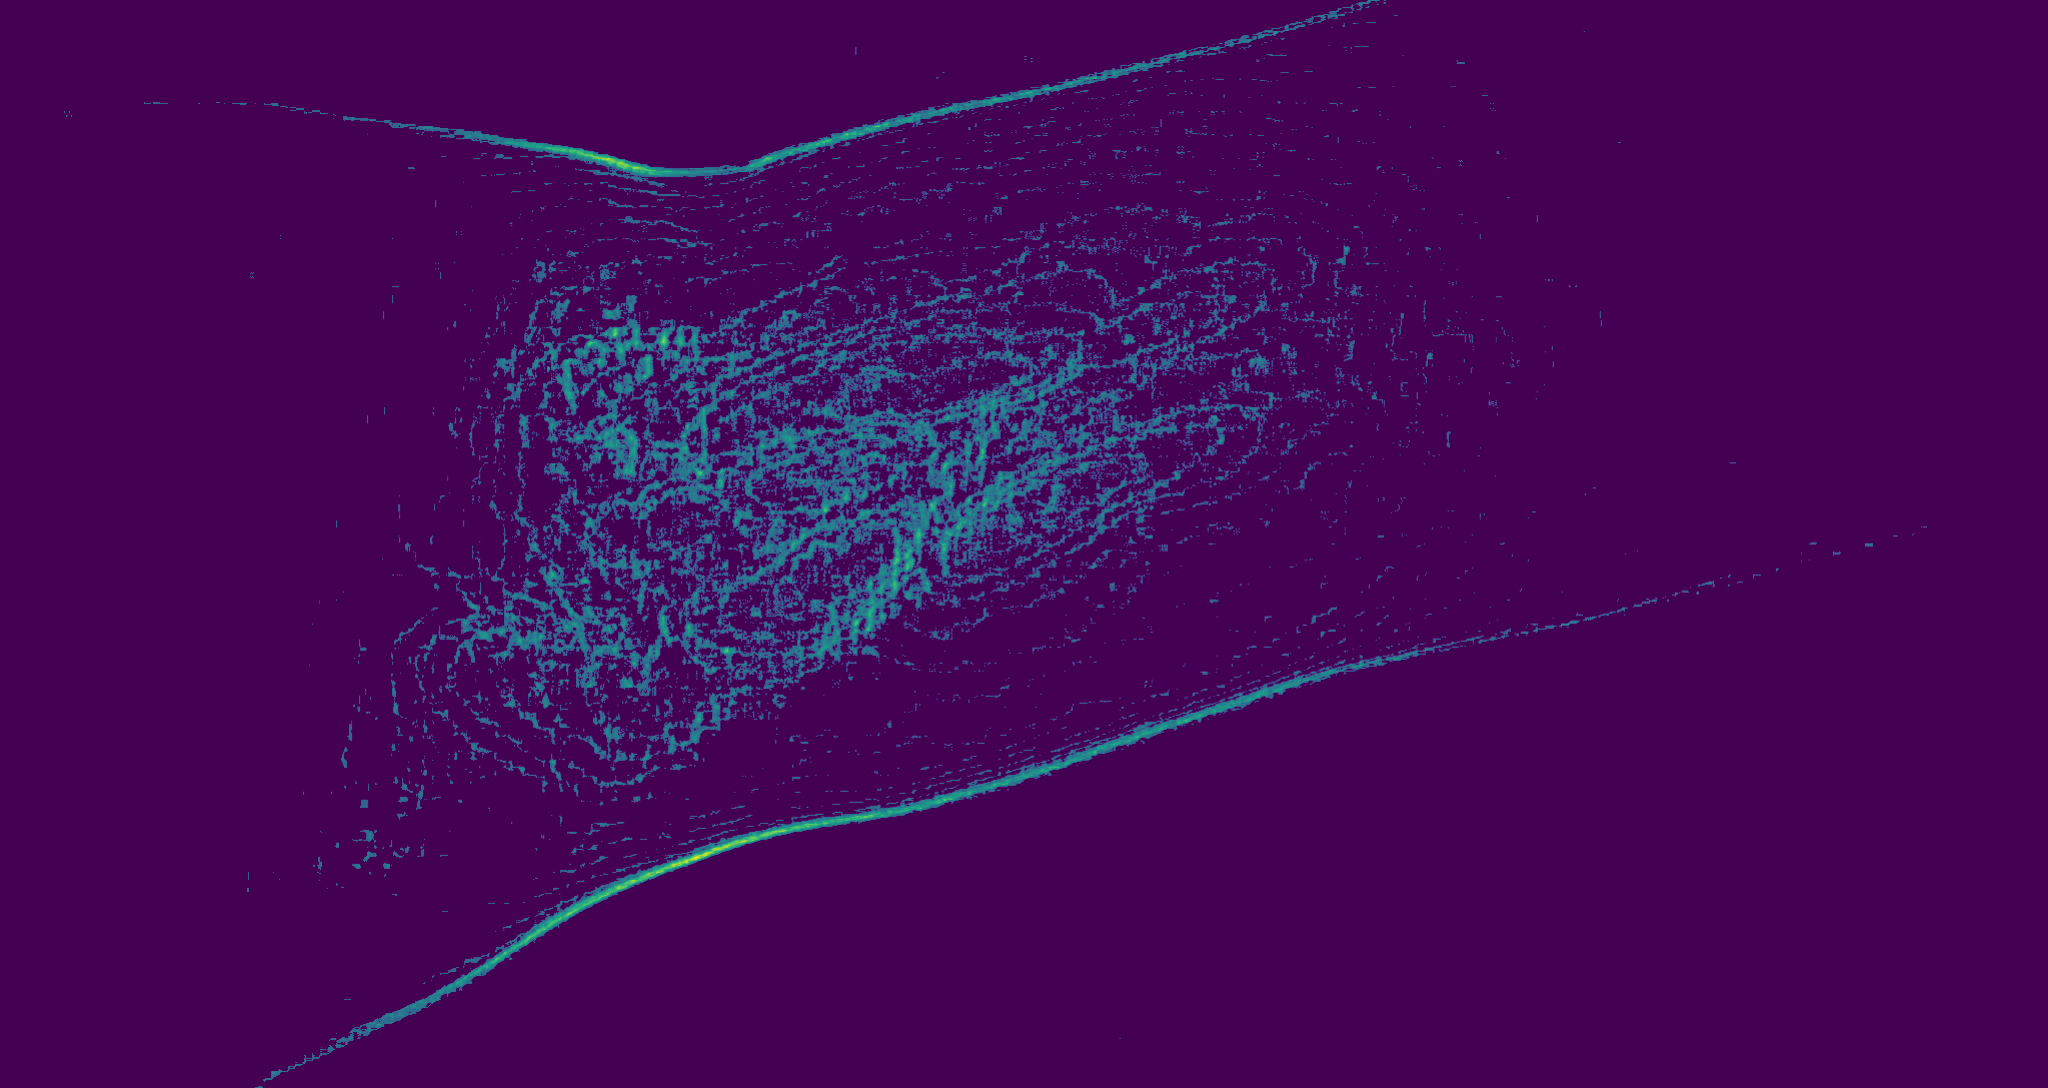
\includegraphics[width=\linewidth]{figures/tp_data7_14.png}
  \end{minipage}
  \hfill
  \begin{minipage}[b]{0.48\textwidth}
    \centering
    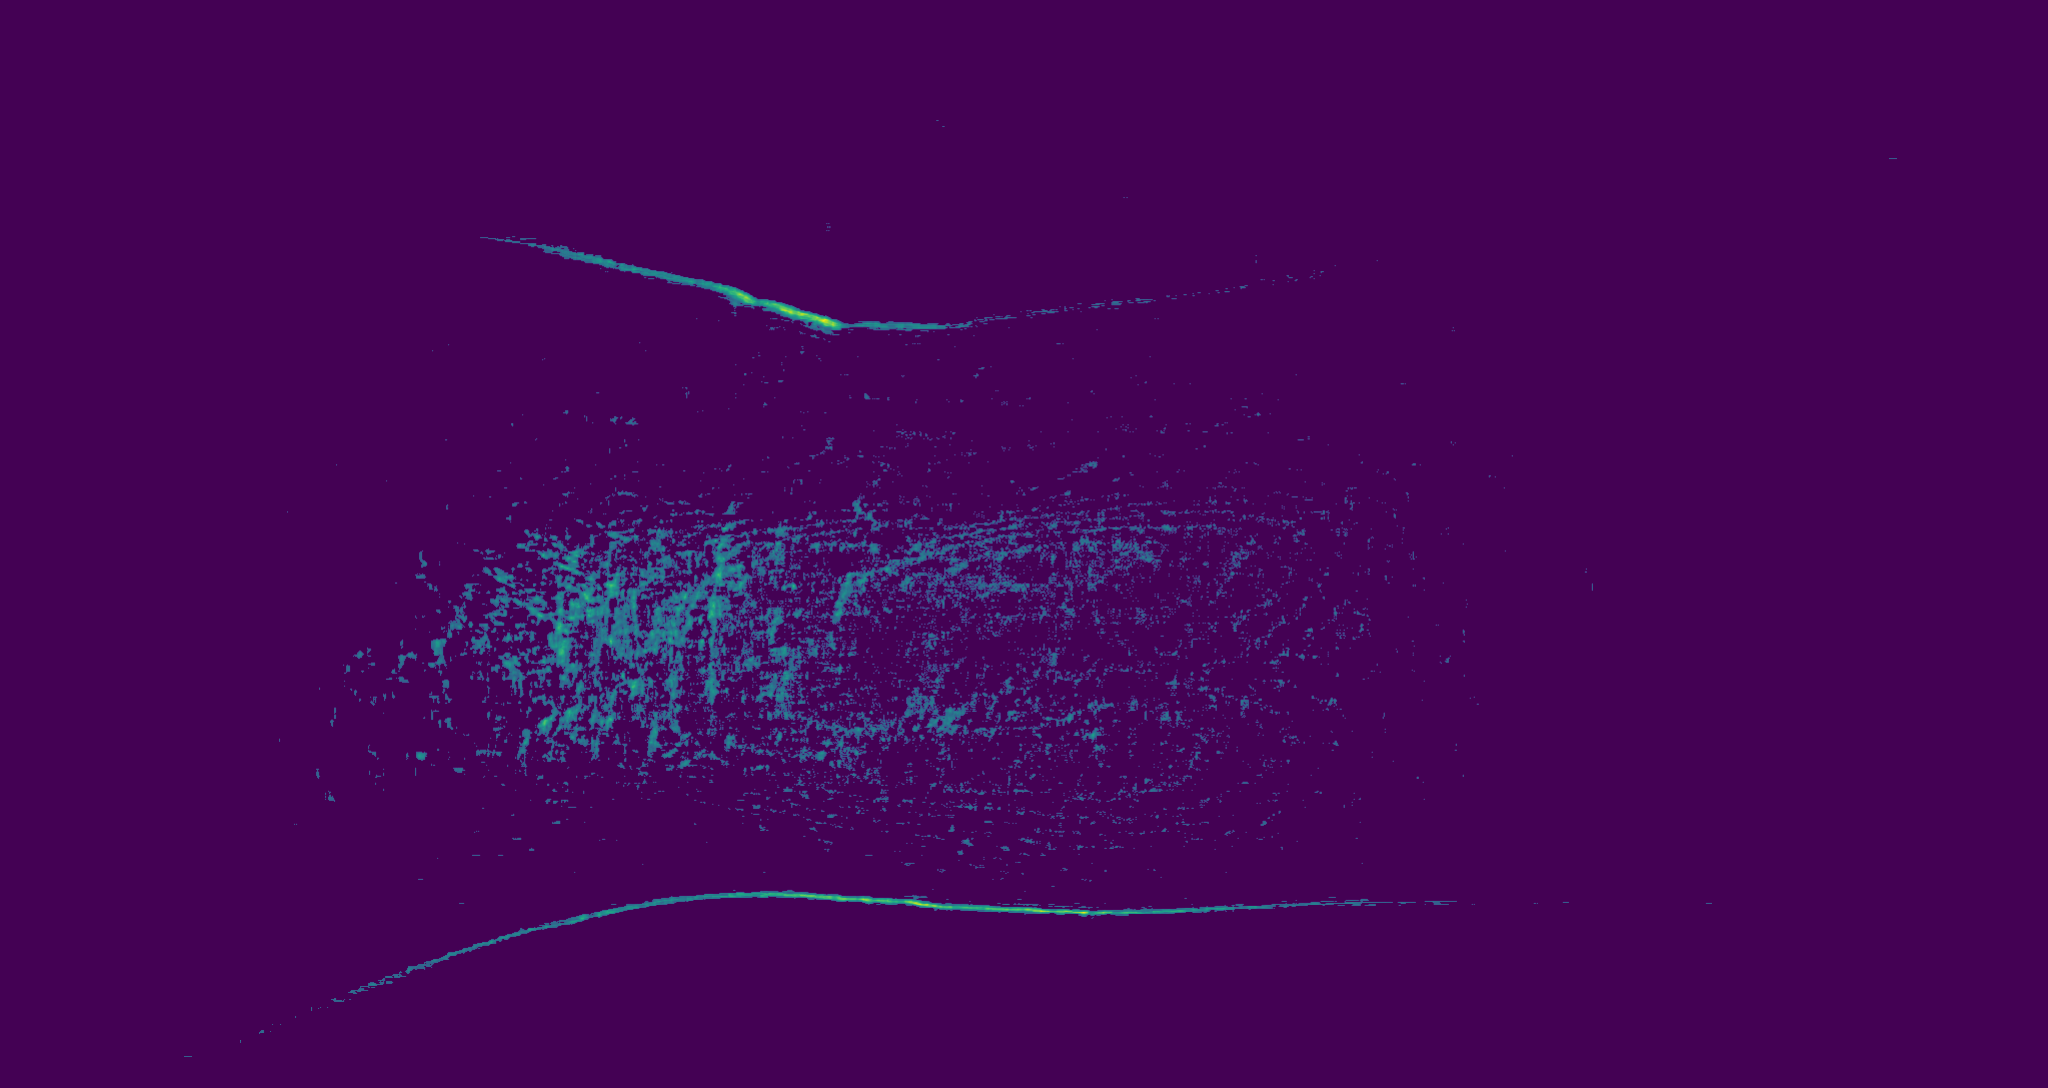
\includegraphics[width=\linewidth]{figures/tp_data9_4.png}
  \end{minipage}
  \\[1ex]
  \begin{minipage}[b]{0.48\textwidth}
    \centering
    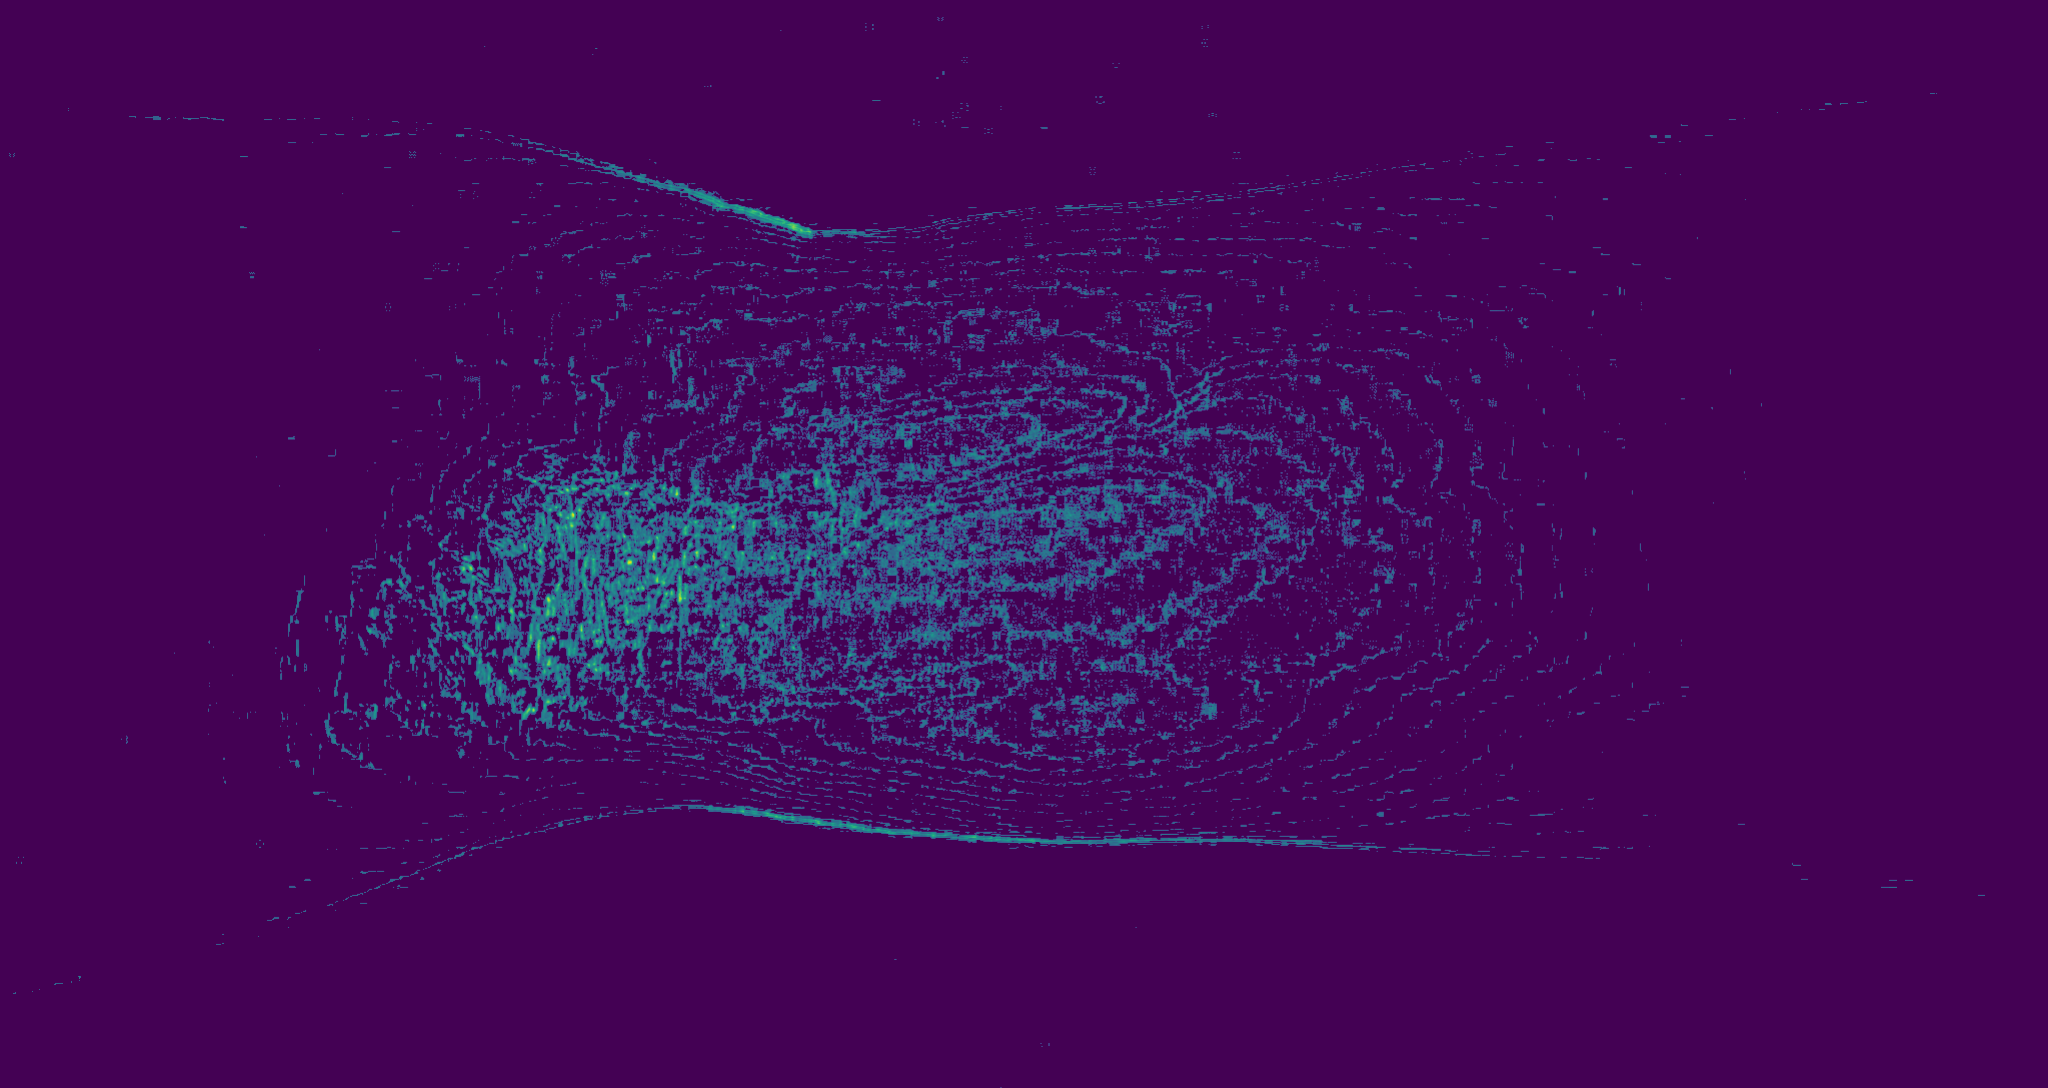
\includegraphics[width=\linewidth]{figures/tp_data9_11.png}
  \end{minipage}
  \hfill
  \begin{minipage}[b]{0.48\textwidth}
    \centering
    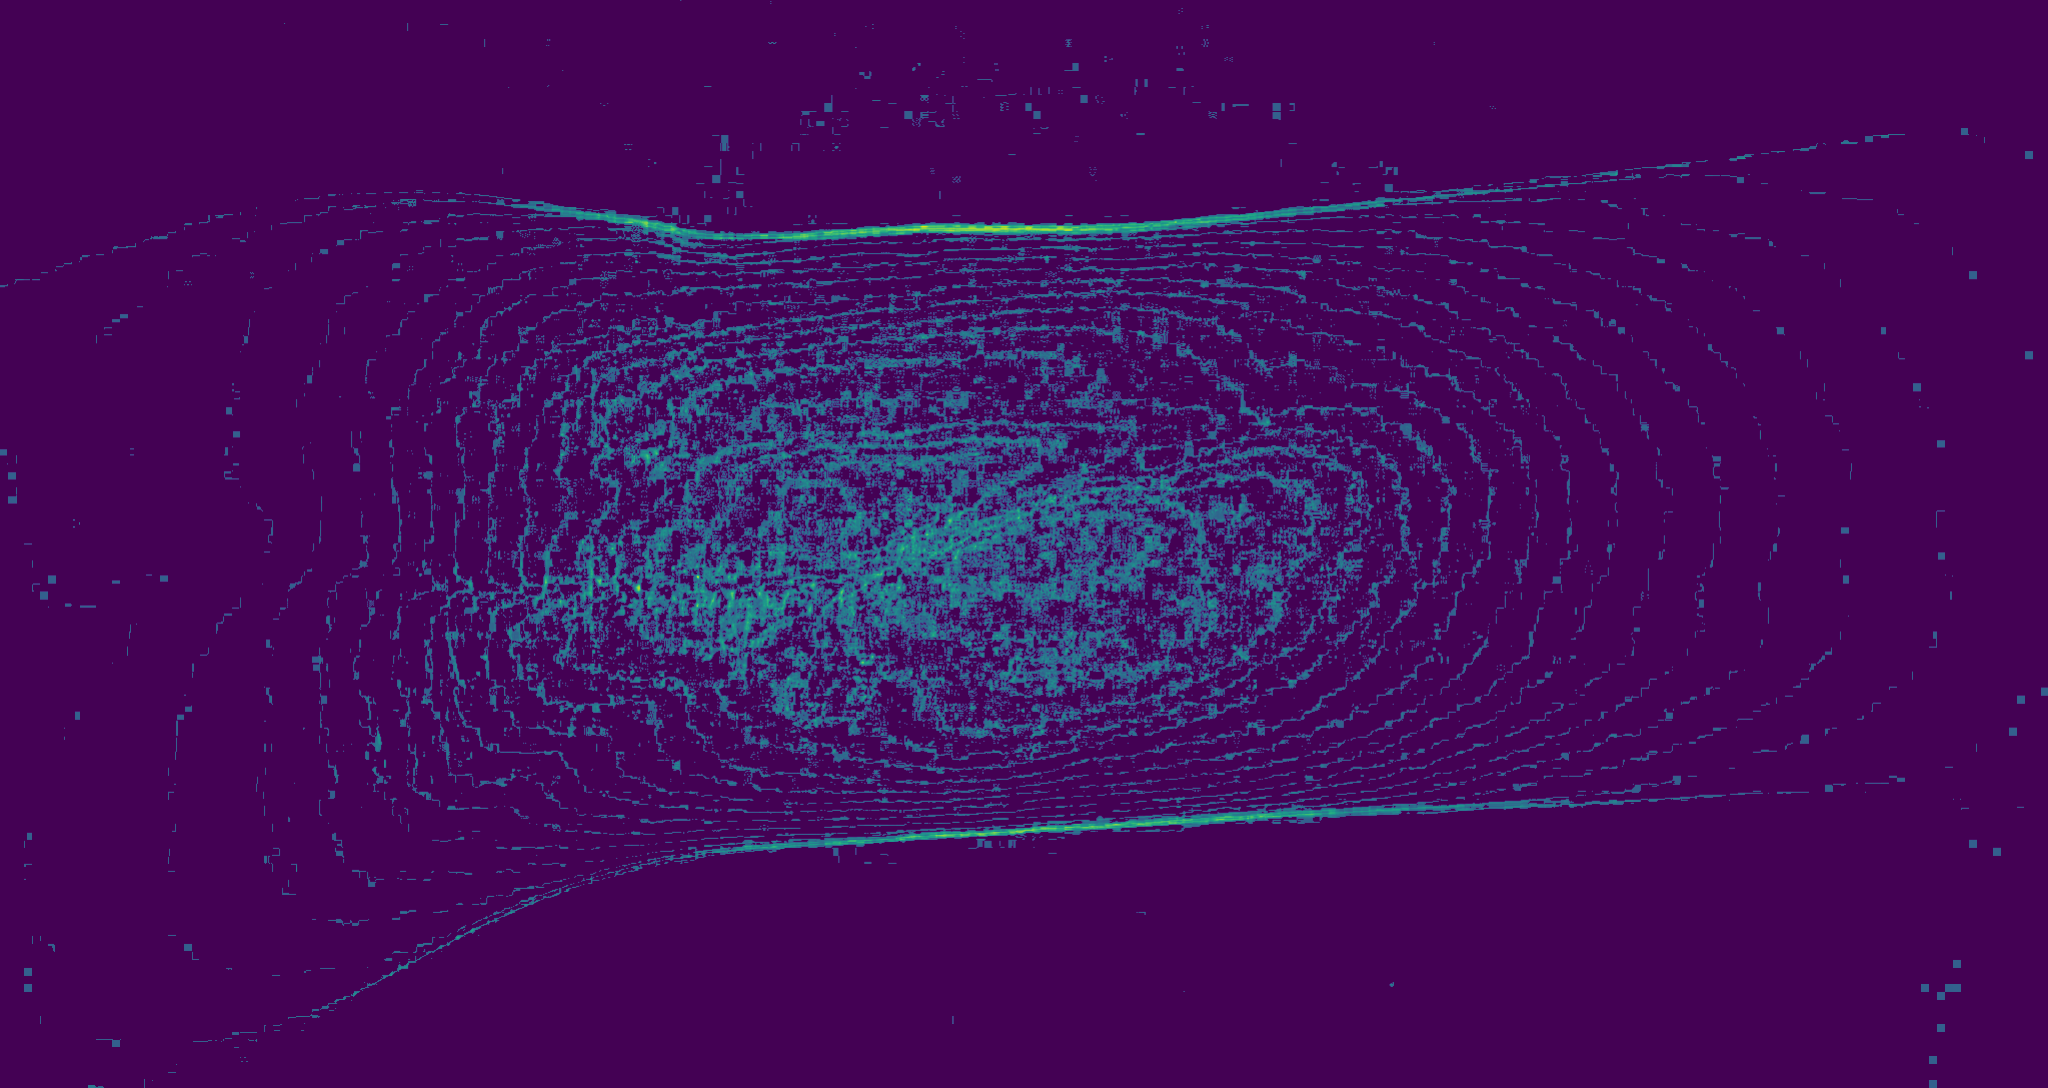
\includegraphics[width=\linewidth]{figures/tp_data16_5.png}
  \end{minipage}
  \caption{temporal prior}
  \label{prior}
\end{figure*}

\subsubsection{Training Details}
We collected a total of 2949 labeled videos and split the dataset into training, validation, and test sets using a 7:2:1 ratio. This results in 2064 training samples, 590 validation samples, and 295 test samples. Each video is annotated with three keypoints corresponding to cun, guan, and chi.

Due to hardware limitations, we downsample the video frames to a resolution of $136 \times 256$ at 30 fps, with a video duration of 3 seconds (90 frames). The model is trained from scratch using the RMSprop optimizer with an initial learning rate of $1 \times 10^{-5}$, which is halved every 10 epochs. The batch size is set to 2, and the network is trained for 100 epochs on an NVIDIA GeForce RTX 3090 GPU.

\subsection{Temporal Attention Prior}
\label{temporal_attention}
The concept of image priors plays a crucial role in computer vision tasks. Image priors refer to assumptions or statistical knowledge about the visual world that can assist in solving various challenges, such as image denoising, segmentation, and restoration. These priors can take many forms, including statistical models, physical constraints, or biological insights. Even in cases with limited training data, incorporating appropriate priors can significantly improve the accuracy and robustness of computer vision systems.

Our proposed temporal attention prior is inspired by Eulerian Video Magnification~\cite{wu2012, wadhwa2013}, which amplifies subtle and otherwise invisible temporal variations—such as guitar string vibrations, facial micro-expressions, and pulse oscillations on the wrist.

The dataset used in this work consists of videos captured at 30 fps, each lasting 3 seconds. Given that human heart rates typically range from 60–90 bpm (i.e., 1 to 1.5 beats per second), each 3-second video captures approximately 3 to 4.5 pulse cycles. Although these weak pulse motions are imperceptible to the human eye, the corresponding gray-level fluctuations can be captured through numerical processing.

To compute the temporal attention prior, we define the set of video frames as $V$, as shown in Equation~\ref{tp1}. We then calculate the average gray value of each spatial location across all frames (Equation~\ref{tp2}). Each frame is subtracted from this mean frame, and the absolute difference is taken to quantify temporal variation (Equation~\ref{tp3}). Next, the differences are summed across time to obtain the attention map (Equation~\ref{tp4}). Finally, a threshold is applied to suppress regions with minimal change (Equation~\ref{tp5}). The resulting temporal attention prior is embedded into the network’s skip connections, and the fusion strategies are further analyzed in the ablation study. Examples of the generated attention maps for different subjects are shown in Figure~\ref{prior}.

\begin{align}
& V=\{V_{N}|N=1, 2, 3...90\},V_{N}\in \mathbb{R}^{1088\times2048}\label{tp1} \\
& M=\frac{\sum_{i=1}^{N} V_{N}}{|V|}, M\in \mathbb{R}^{1088\times2048}\label{tp2} \\
& D=\{D_{N}||V_{N}-M|, V_{N}\in V\}, D\in \mathbb{R}^{1088\times2048}\label{tp3} \\
& S=\sum_{i=1}^{N} D_{N}, S\in \mathbb{R}^{1088\times2048}\label{tp4} \\
& T=S > Threshold, T\in \mathbb{R}^{1088\times2048}\label{tp5}
\end{align}
% 2025-08-04

\section{Experiments}
In this section, we evaluate the effectiveness of our proposed heatmap-based method with a temporal attention prior for localizing the three pulse positions: cun, guan, and chi. We begin by detailing the experimental setup, followed by ablation studies on temporal attention fusion strategies and keypoint fitting methods. We then compare our approach against several existing keypoint detection models and, finally, analyze the trade-offs between regression-based and heatmap-based frameworks.

\subsection{Experimental Setup}
All experiments are conducted on a dataset comprising 2949 infrared wrist videos, each annotated with three keypoints corresponding to the pulse positions: cun, guan, and chi. The dataset is divided into training, validation, and test sets using a 7:2:1 split, resulting in 2064, 590, and 295 samples, respectively. Each video consists of 90 grayscale frames with a resolution of $136 \times 256$ pixels and a frame rate of 30 frames per second (fps). To reduce computational overhead, the video frames are treated as single-channel images, forming an input tensor of shape $(90, 136, 256)$. All models are trained from scratch using the RMSprop optimizer with an initial learning rate of $1 \times 10^{-5}$, which is reduced by a factor of 0.5 every 10 epochs. Training is performed for 100 epochs with a batch size of 4 on an NVIDIA GeForce RTX 3090 GPU. We evaluate the model's performance using three metrics: the average distance error ($D$), the overall average error ($F$), and the accuracy within pixel thresholds of 100, 80, 60, 40, and 20 pixels, which correspond to physical distances of 10, 8, 6, 4, and 2 millimeters, respectively.
% 2025-08-07

\subsection{Ablation on Temporal Attention Fusion}
We investigate the effectiveness of different fusion strategies for incorporating the temporal attention prior into the network. Specifically, we compare direct addition at the encoder with three decoder-side strategies: addition, multiplication, and concatenation, all performed after convolution. As shown in Table~\ref{tab:fusion-strategy-comparison}, fusing the prior at the encoder significantly degrades performance, likely due to the loss of fine-grained spatial information from downsampling. In contrast, decoder-side fusion preserves spatial resolution, with the concatenation strategy achieving the highest accuracy at finer thresholds—surpassing 24\% accuracy at the 2mm (20-pixel) threshold. Based on these results, we adopt the decoder-side concatenation strategy for all subsequent experiments.

\begin{table*}[htbp!]
    \centering
    \caption{Comparison of Different Fusion Strategies}
    \setlength{\tabcolsep}{3pt}{
    \begin{tabular}{|c|c|c|c|c|c|c|c|c|}
        \hline
        \multirow{2}{*}{Fusion Strategy}
        &\multirow{2}{*}{\makecell[c]{Keypoint\\Name}}
        &\multirow{2}{*}{\makecell[c]{Average\\Error $D$}}
        &\multirow{2}{*}{\makecell[c]{Overall\\Error $F$}}
        &\multicolumn{5}{c|}{Accuracy at Each Threshold (\%)}
        \\
        \cline{5-9}
        & & & &100 px &80 px &60 px &40 px &20 px
        \\
        \hline
        \multirow{3}{*}{\makecell[c]{Addition\\in\\Encoder}}
        &Cun &52.254 & &94.237 &88.814 &76.271 &45.085 &16.610\\
        &Guan &71.456 &70.402 &89.492 &84.407 &70.508 &50.847 &20.000\\
        &Chi &87.496 & &86.780 &79.661 &64.407 &42.373 &14.237\\
        \hline
        \multirow{3}{*}{\makecell[c]{Direct\\Addition\\in Decoder}}
        &Cun &38.290 & &98.305 &94.237 &84.407 &60.000 &\textbf{23.051}\\
        &Guan &39.436 &42.653 &\textbf{97.288} &93.898 &84.746 &60.678 &20.678\\
        &Chi &50.232 & &96.271 &90.169 &77.627 &55.932 &20.678\\
        \hline
        \multirow{3}{*}{\makecell[c]{Addition\\after\\Convolution in Decoder}}
        &Cun &\textbf{37.637} & &\textbf{99.322} &95.254 &85.763 &\textbf{63.390} &21.695\\
        &Guan &38.665 &41.645 &97.288 &93.220 &85.763 &61.017 &21.695\\
        &Chi &48.632 & &94.915 &88.814 &76.610 &53.559 &20.339\\
        \hline
        \multirow{3}{*}{\makecell[c]{Multiplication\\after\\Convolution in Decoder}}
        &Cun &37.956 & &98.983 &\textbf{96.949} &84.746 &59.661 &20.678\\
        &Guan &37.785 &40.453 &97.288 &\textbf{94.576} &84.407 &61.695 &24.068\\
        &Chi &45.616 & &94.237 &88.475 &76.949 &51.864 &15.932\\
        \hline
        \multirow{3}{*}{\makecell[c]{Concatenation\\after\\Convolution in Decoder}}
        &Cun &42.442 & &98.305 &96.271 &\textbf{87.119} &62.712 &20.339\\
        &Guan &\textbf{36.803} &\textbf{40.257} &96.610 &93.220 &\textbf{86.441} &\textbf{65.085} &\textbf{24.407}\\
        &Chi &\textbf{41.527} & &\textbf{97.288} &\textbf{90.508} &\textbf{78.983} &\textbf{57.966} &\textbf{22.034}\\
        \hline
    \end{tabular}}
    \label{tab:fusion-strategy-comparison}
\end{table*}

\begin{table*}[htbp!]
    \centering
    \caption{Performance Comparison of Keypoint Fitting Strategies}
    \setlength{\tabcolsep}{3pt}{
    \begin{tabular}{|c|c|c|c|c|c|c|c|c|}
        \hline
        \multirow{2}{*}{\makecell[c]{Fitting\\Method}}
        &\multirow{2}{*}{\makecell[c]{Keypoint\\Name}}
        &\multirow{2}{*}{\makecell[c]{Average\\Error $D$}}
        &\multirow{2}{*}{\makecell[c]{Overall\\Error $F$}}
        &\multicolumn{5}{c|}{Accuracy at Different Thresholds (\%)} \\
        \cline{5-9}
        & & & &100 pixels &80 pixels &60 pixels &40 pixels &20 pixels \\
        \hline
        \multirow{3}{*}{\makecell[c]{Maximum Value}}
        &Cun &\textbf{42.442} & &\textbf{98.305} &96.271 &87.119 &62.712 &20.339\\
        &Guan &36.803 &40.257 &96.610 &93.220 &86.441 &65.085 &24.407\\
        &Chi &41.527 & &97.288 &90.508 &78.983 &57.966 &\textbf{22.034}\\
        \hline
        \multirow{3}{*}{\makecell[c]{Circular Region\\Expectation}}
        &Cun &44.126 & &97.966 &\textbf{96.949} &\textbf{87.458} &\textbf{63.051} &\textbf{24.407}\\
        &Guan &\textbf{35.679} &\textbf{40.198} &\textbf{97.288} &\textbf{93.559} &\textbf{87.119} &\textbf{67.119} &\textbf{26.441}\\
        &Chi &\textbf{40.788} & &\textbf{97.627} &\textbf{91.186} &\textbf{80.339} &\textbf{58.305} &21.356\\
        \hline
    \end{tabular}}
    \label{tab:keypoint-fitting-comparison}
\end{table*}

\subsection{Comparison of Keypoint Fitting Strategies}
A common approach for keypoint localization using heatmaps is to take the coordinate of the maximum probability value, as shown in Equation~\ref{fit-1}, where $C_{max}$ denotes the coordinate of the maximum value, $argmax$ represents the index of the maximum value, $V$ is the flattened one-dimensional representation of the heatmap, and $H$ and $W$ are the height and width of the image, respectively. However, since pixel indices in the image space are integers, directly using the peak of the heatmap may result in localization bias. For example, in our case, the image resolution is $136\times256$, and after four downsampling operations, the feature map is reduced to $8\times16$. If a keypoint is originally located at (117, 117), its downsampled coordinate becomes (7, 7), and after upsampling, it is restored to (112, 112), resulting in a 5-pixel error.

To address this issue, we adopt an alternative keypoint fitting strategy—center of mass within a circular region. Specifically, we take the point with the highest probability as the center, and compute the expectation of coordinates within a unit circle weighted by their probability values, as defined in Equation~\ref{fit-2}. Let $V$ denote the flattened heatmap with spatial size $H \times W$.

\begin{align}
& C_{max}=(\frac{argmax(V)}{W}, \, argmax(V) \mod W) \label{fit-1}\\
& E(C_{max})=\frac{\sum_{(x, y) \in \text{circle}}(x, y)P_{x, y}}{\sum_{(x, y) \in \text{circle}}P_{x, y}} \label{fit-2}
\end{align}

Here, $(x, y)$ denotes the pixel coordinates within the unit circle, and $P_{x, y}$ represents the probability at coordinate $(x, y)$. As shown in Table~\ref{tab:keypoint-fitting-comparison}, the Circular Region Expectation method outperforms the Maximum Value approach in most metrics, confirming its effectiveness for precise keypoint localization.
% 2025-08-07

% \subsection{Effect of Temporal Attention Prior}
% To visualize the impact of the temporal attention prior, we extract and compare the final upsampled feature maps from U-Net and our PLNTP. As shown in Figures~\ref{U-Net特征图} and~\ref{U-Net + 时序注意力先验特征图}, our method enhances activation in wrist regions while suppressing background noise, indicating improved focus on relevant spatial-temporal features.

\begin{table*}[t]
    \centering
    \caption{Comparison of the Proposed Method and Other Heatmap-Based Models in Localization Accuracy}
    \resizebox{\textwidth}{!}{%
    \setlength{\tabcolsep}{1pt}%
    \begin{tabular}{|c|c|c|c|c|c|c|c|c|c|}
        \hline
        \multirow{2}{*}{Model Name}
        &\multirow{2}{*}{\makecell[c]{Parameter\\Count}}
        &\multirow{2}{*}{\makecell[c]{Keypoint\\Name}}
        &\multirow{2}{*}{\makecell[c]{Average\\Error $D$}}
        &\multirow{2}{*}{\makecell[c]{Overall\\Error $F$}}
        &\multicolumn{5}{c|}{Accuracy at Each Threshold for Cun, Guan, and Chi (\%)}
        \\
        \cline{6-10}
        & & & & &100 px &80 px &60 px &40 px &20 px
        \\
        \hline
        \multirow{3}{*}{\makecell[c]{Hourglass\cite{newell2016}}}
        & &Cun &73.587 & &89.492 &84.407 &73.559 &47.458 &12.203\\
        &56M &Guan &51.808 &66.910 &91.864 &85.763 &71.864 &50.847 &17.288\\
        & &Chi &75.334 & &87.797 &80.678 &68.475 &41.017 &13.559\\
        \hline
        \multirow{3}{*}{\makecell[c]{CPN\cite{chen2018}}}
        & &Cun &56.184 & &89.153 &82.034 &66.441 &37.966 &13.898\\
        &110M &Guan &56.813 &61.640 &86.102 &79.322 &63.051 &43.729 &15.254\\
        & &Chi &71.923 & &83.390 &75.932 &59.322 &37.627 &15.254\\
        \hline
        \multirow{3}{*}{\makecell[c]{Flat-net\cite{eslami2020}}}
        & &Cun &79.291 & &76.271 &68.136 &54.576 &33.559 &8.814\\
        &4M &Guan &83.374 &84.949 &69.492 &59.322 &44.407 &25.763 &9.492\\
        & &Chi &92.183 & &65.424 &52.881 &38.644 &20.678 &6.780\\
        \hline
        \multirow{3}{*}{\makecell[c]{RSN\cite{cai2020}}}
        & &Cun &128.447 & &77.288 &72.203 &64.746 &41.695 &14.576\\
        &105M &Guan &95.640 &104.391 &76.949 &70.847 &62.373 &45.763 &16.271\\
        & &Chi &89.087 & &74.915 &70.169 &58.644 &39.661 &13.898\\
        \hline
        \multirow{3}{*}{\makecell[c]{SFCN\cite{yang2022}}}
        & &Cun &1241.108 & &0 &0 &0 &0 &0\\
        &13M &Guan &1023.622 &1151.304 &0 &0 &0 &0 &0\\
        & &Chi &1189.180 & &0 &0 &0 &0 &0\\
        \hline
        \multirow{3}{*}{\makecell[c]{U-Net\cite{ronneberger2015}}}
        & &Cun &\textbf{41.871} & &\textbf{98.644} &94.576 &83.390 &56.949 &15.932\\
        &39M &Guan &38.710 &42.501 &\textbf{97.966} &92.881 &84.746 &60.000 &20.000\\
        & &Chi &46.921 & &95.593 &90.847 &76.949 &51.864 &19.322\\
        \hline
        \multirow{3}{*}{\makecell[c]{U-Net\\+\\Temporal Attention Prior}}
        & &Cun &44.130 & &97.966 &\textbf{96.949} &\textbf{87.458} &\textbf{63.051} &\textbf{24.407}\\
        &51M &Guan &\textbf{35.680} &\textbf{40.198} &97.288 &\textbf{93.559} &\textbf{87.119} &\textbf{67.119} &\textbf{26.441}\\
        & &Chi &\textbf{40.790} & &\textbf{97.627} &\textbf{91.186} &\textbf{80.339} &\textbf{58.305} &\textbf{21.356}\\
        \hline
    \end{tabular}}
    \label{tab:comparison-with-other-models}
\end{table*}

\begin{table*}[htbp!]
    \centering
    \caption{Comparison Between Regression-Based and Heatmap-Based Methods}
    \resizebox{\textwidth}{!}{%
    \setlength{\tabcolsep}{1pt}%
    \begin{tabular}{|c|c|c|c|c|c|c|c|c|c|c|}
        \hline
        \multirow{2}{*}{Model Type}
        &\multirow{2}{*}{\makecell[c]{Param\\Count}}
        &\multirow{2}{*}{\makecell[c]{Inference\\Time (ms)}}
        &\multirow{2}{*}{\makecell[c]{Keypoint\\Name}}
        &\multirow{2}{*}{\makecell[c]{Average\\Error $D$}}
        &\multirow{2}{*}{\makecell[c]{Overall\\Error $F$}}
        &\multicolumn{5}{c|}{Accuracy at Each Threshold for Cun, Guan, and Chi (\%)}
        \\
        \cline{7-11}
        & & & & & &100 px &80 px &60 px &40 px &20 px
        \\
        \hline
        \multirow{3}{*}{\makecell[c]{Regression-Based}}
        & & &Cun &\textbf{39.810} & &\textbf{98.983} &\textbf{97.627} &81.695 &55.254 &15.593\\
        &146M &\textbf{501} &Guan &39.818 &40.942 &\textbf{98.644} &\textbf{96.949} &81.107 &56.271 &19.322\\
        & & &Chi &43.200 & &\textbf{98.983} &\textbf{92.542} &75.593 &49.831 &16.949\\
        \hline
        \multirow{3}{*}{\makecell[c]{Heatmap-Based}}
        & & &Cun &44.130 & &97.966 &96.949 &\textbf{87.458} &\textbf{63.051} &\textbf{24.407}\\
        &51M &1541 &Guan &\textbf{35.680} &\textbf{40.198} &97.288 &93.559 &\textbf{87.119} &\textbf{67.119} &\textbf{26.441}\\
        & & &Chi &\textbf{40.790} & &97.627 &91.186 &\textbf{80.339} &\textbf{58.305} &\textbf{21.356}\\
        \hline
    \end{tabular}}
    \label{tab:comparison-regression-vs-heatmap}
\end{table*}


\subsection{Comparison with Existing Methods}
We compare our method against state-of-the-art heatmap-based models including Hourglass~\cite{newell2016}, CPN~\cite{chen2018}, Flat-net~\cite{eslami2020}, RSN~\cite{cai2020}, and SFCN~\cite{yang2022}. As shown in Table~\ref{tab:comparison-with-other-models}, our method outperforms all baselines at finer thresholds. For example, at the 2mm threshold, our model achieves 24.4\%, 26.4\%, and 21.3\% accuracy for cun, guan, and chi, respectively—significantly higher than all other models.

\subsection{Heatmap-based vs Regression-based Comparison}
We also compare our method to a regression-based baseline. Table~\ref{tab:comparison-regression-vs-heatmap} shows that while the regression-based method achieves faster inference and better accuracy at coarse thresholds, our heatmap-based method excels at fine-grained localization (i.e., under 60 pixels). Therefore, we recommend regression-based methods for real-time, low-precision scenarios like wearable devices, and our heatmap-based approach for high-precision tasks such as clinical-grade pulse diagnosis instruments.

% \subsection{Qualitative Results}
% Figure~\ref{基于热度图的网络定位效果可视化} presents qualitative results of our model. Red dots represent ground truth keypoints, blue dots denote predictions, and green circles indicate the 60-pixel tolerance zone. The predictions show that our model can precisely locate all three pulse points even in challenging cases with subtle pulse signals.
% 2025-08-12

\section{Conclusion}
In this work, we proposed PLNTP, a heatmap-based network with a temporal attention prior, to simultaneously localize the three pulse positions—cun, guan, and chi—on infrared wrist videos. Inspired by the subtle periodic motion of the pulse, we designed a lightweight and effective temporal attention prior that enhances the model’s spatial-temporal feature representation without increasing model parameters.

We conducted comprehensive experiments to evaluate the effectiveness of our method. Ablation studies showed that fusing the temporal attention prior at the decoder via convolutional concatenation significantly improved localization accuracy, especially under strict thresholds. Additionally, we introduced a keypoint fitting strategy based on regional probability expectation, which further reduced localization error compared to the conventional maximum activation method.

Compared with existing state-of-the-art heatmap-based models, our method achieved superior accuracy at fine localization thresholds, demonstrating its robustness and effectiveness. Furthermore, we analyzed the trade-offs between regression-based and heatmap-based approaches and concluded that our method is more suitable for high-precision applications such as clinical pulse diagnosis instruments.

Overall, this research highlights the potential of combining deep learning with temporal prior knowledge to advance intelligent Traditional Chinese Medicine (TCM) diagnosis. Future work may focus on real-time implementation and exploring personalized modeling for different wrist morphologies.

\bibliographystyle{plain}
\bibliography{reference}
\end{document}
% 2025-08-12